\chapter{Desarrollo}

\section{Diseño general del sistema}
El sistema fue diseñado para gestionar información de deportistas de forma simple y modular, permitiendo generar datos, cargarlos desde archivos CSV y aplicar sobre ellos distintas operaciones de ordenamiento, búsqueda y análisis experimental. Para facilitar su desarrollo y comprensión, la implementación se organizó en componentes que separan la representación de los datos, la generación y carga de registros, y las funcionalidades principales ofrecidas por el programa.
\subsection{Estructura de datos de los deportistas}
La estructura de datos utilizada para representar a cada deportista se definió como una estructura con campos específicos para almacenar distinta información; estos campos corresponden a:
\begin{itemize}
    \item \texttt{ID:} Identificador único del deportista.
    \item \texttt{Nombre:} Nombre completo del deportista.
    \item \texttt{Equipo:} Equipo al que pertenece.
    \item \texttt{Puntaje:} Puntuación total acumulada.
    \item \texttt{Competencias:} Número de competencias en las que ha participado.
\end{itemize}
Cada parámetro permite almacenar información, la cual puede ser utilizada para ordenar o buscar a los deportistas según distintos criterios. Esta estructura se implementó utilizando un \texttt{struct} en C, lo que facilita su manejo y acceso a los campos correspondientes durante las operaciones de ordenamiento y búsqueda.

\subsection{Generación y carga de datos}
La generación de datos de los parámetros asociados a deportistas se realizó mediante distintas funciones, las cuales permiten crear u obtener estos registros de manera pseudoaleatoria. La generación de un nombre se realizó permitiendo seleccionar aleatoriamente letras de un conjunto predefinido, escogiendo un tamaño de 3 a 8 caracteres. Para el equipo, se seleccionó aleatoriamente entre un conjunto específico de equipos de Esports. El ID se generó en forma incremental, asegurando la unicidad de cada registro. Por otro lado, el puntaje y la cantidad de competencias se generaron utilizando funciones de generación de números aleatorios dentro de rangos predefinidos. Esta metodología permitió crear un conjunto de datos variado y representativo para probar las funcionalidades del sistema. Posterior a la creación de los registros, estos se desordenaron utilizando el algoritmo de Fisher-Yates para garantizar que los datos no se encuentren en un orden específico, lo que es fundamental para evaluar correctamente el desempeño de los algoritmos de ordenamiento y búsqueda implementados. Finalmente, los registros generados se almacenaron en un archivo CSV, lo que facilita su posterior carga y manipulación dentro del programa.


\subsection{Funcionalidades del sistema}
Una vez cargados los datos de los deportistas, el programa permite realizar distintas operaciones combinando opciones de línea de comandos con menús interactivos. Entre las funcionalidades principales se encuentra el ordenamiento de los datos de los deportistas de manera ascendente o descendente utilizando el ID, puntaje, cantidad de competencias, nombre y equipo. Para ello, el usuario puede seleccionar alguno de los algoritmos de ordenamiento implementados en el programa.

Otra funcionalidad importante es la búsqueda de deportistas por ID, la cual puede realizarse mediante búsqueda secuencial o búsqueda binaria iterativa. Esto permite comparar no solo la correctitud de ambos métodos, sino también su desempeño bajo distintas condiciones de entrada.

Además, el sistema permite mostrar un ranking con los mejores \(N\) deportistas de acuerdo a su puntaje, lo que logra una aplicación práctica del ordenamiento de datos dentro del contexto del problema planteado.

Junto con las operaciones anteriores, el programa incorpora la ejecución de benchmarks para medir el tiempo de ejecución de los algoritmos de ordenamiento y búsqueda. Estos resultados se almacenan en archivos CSV y posteriormente pueden utilizarse para generar gráficos comparativos mediante gnuplot, facilitando el análisis experimental de los algoritmos implementados.

En conjunto, estas funcionalidades permiten que el sistema no solo cumpla con los requerimientos prácticos de manipulación de datos, sino que también sirva como base para el estudio comparativo del comportamiento de los algoritmos.
\section{Implementación de algoritmos de ordenamiento}
Para el procesamiento de los datos de deportistas, el sistema incorpora distintos algoritmos de ordenamiento iterativos, cada uno con características particulares en cuanto a funcionamiento y rendimiento. Su implementación permite ordenar los datos según diversos criterios y, al mismo tiempo, comparar su comportamiento en distintos casos de prueba desde un punto de vista teórico y experimental.


\subsection{Bubble Sort optimizado}\label{subsec:bubblesort}
Bubble Sort es un algoritmo de ordenamiento iterativo que se basa en comparar elementos adyacentes y realizar intercambios si están en el orden incorrecto. En su versión optimizada, se introduce una bandera para detectar si se realizaron intercambios durante una pasada completa. Si no se realizaron intercambios, significa que el arreglo ya está ordenado, lo que permite finalizar el proceso antes de completar todas las pasadas necesarias en la versión estándar.

Su implementación permite ordenar los registros de deportistas según distintos campos, como ID, puntaje, competencias, nombre y equipo. En el mejor caso, cuando los datos ya están ordenados, Bubble Sort optimizado tiene una complejidad temporal de \(O(n)\) debido a que solo realiza una pasada para verificar el orden. Sin embargo, en el caso promedio y peor caso, su complejidad es \(O(n^2)\) debido a la necesidad de realizar múltiples pasadas y comparaciones para ordenar completamente el arreglo.

\subsection{Insertion Sort}
Insertion Sort es un algoritmo de ordenamiento iterativo que construye gradualmente una porción ordenada del arreglo. Su funcionamiento consiste en tomar cada elemento y ubicarlo en la posición que le corresponde dentro de los elementos previamente ordenados, desplazando hacia la derecha aquellos que sean mayores o menores según el criterio de orden elegido.

En este proyecto, su implementación permite ordenar los registros de deportistas de acuerdo con distintos campos, como ID, puntaje, competencias, nombre y equipo.

Una de las ventajas de Insertion Sort es su buen desempeño cuando los datos ya se encuentran ordenados o casi ordenados, ya que en esos casos realiza pocos desplazamientos. En cambio, cuando la entrada se encuentra en el peor caso, su cantidad de comparaciones y movimientos aumenta considerablemente.

Teóricamente, Insertion Sort presenta complejidad \(O(n)\) en el mejor caso y \(O(n^2)\) tanto en el caso promedio como en el peor caso.

\subsection{Selection Sort optimizado}
Selection Sort es un algoritmo de ordenamiento iterativo que se basa en seleccionar el elemento mínimo (o máximo) de la porción no ordenada del arreglo y colocarlo en su posición correcta. En su versión optimizada, se realiza una sola pasada para encontrar tanto el mínimo como el máximo en cada iteración, lo que reduce la cantidad de pasadas necesarias para ordenar completamente el arreglo.
En este proyecto, al igual que los demás algoritmos, se implementó para ordenar los registros de deportistas según distintos criterios.

La optimización de Selection Sort permite reducir el número de pasadas externas al ubicar simultáneamente los extremos del segmento no ordenado. Sin embargo, su complejidad temporal sigue siendo \(O(n^2)\) en el mejor, promedio y peor caso, debido a que la cantidad de comparaciones continúa creciendo de forma cuadrática con el tamaño de la entrada.

\subsection{Cocktail Shaker Sort}
Este algoritmo corresponde a una variación de Bubble Sort (\ref{subsec:bubblesort}) que recorre el arreglo en ambas direcciones durante cada iteración. Primero desplaza los elementos más grandes hacia el final y, posteriormente, mueve los más pequeños hacia el inicio. Esta característica lo vuelve especialmente útil cuando la entrada se encuentra parcialmente invertida, ya que permite corregir desórdenes en ambos extremos dentro de una misma iteración externa.

En esta implementación, si durante la pasada hacia adelante no se detectan intercambios, el algoritmo finaliza inmediatamente. Por ello, su mejor caso también es \(O(n)\). No obstante, en el caso promedio y en el peor caso conserva complejidad \(O(n^2)\), y en la práctica suele presentar una sobrecarga constante mayor que Bubble Sort optimizado e Insertion Sort debido al doble recorrido que realiza cuando la entrada aún no está ordenada.

Al igual que los demás algoritmos de ordenamiento implementados en este proyecto, Cocktail Shaker Sort es capaz de ordenar los registros de deportistas según distintos criterios y sentidos, lo que permite evaluar su desempeño en función de la disposición inicial de los datos y compararlo con otras estrategias de ordenamiento.

\section{Implementación de algoritmos de búsqueda}
Además de ordenar los datos, el sistema permite localizar deportistas específicos a partir de su ID mediante algoritmos de búsqueda iterativos. Para ello se implementaron dos enfoques distintos, lo que permite comparar una estrategia de búsqueda directa sobre datos no ordenados con otra más eficiente que requiere un arreglo previamente ordenado.

\subsection{Búsqueda secuencial}
La búsqueda secuencial consiste en recorrer los elementos del arreglo uno a uno hasta encontrar el valor buscado o llegar al final de la estructura. En este proyecto, su implementación se utiliza para localizar deportistas a partir de su ID, comparando el identificador buscado con el ID de cada registro almacenado en memoria.

Una de las principales ventajas de este método es su simplicidad, ya que no requiere que los datos se encuentren previamente ordenados. Esto la convierte en una alternativa directa para trabajar sobre el arreglo cargado desde el archivo CSV. Sin embargo, su rendimiento depende de la posición del elemento buscado, y en el peor caso debe revisar todos los registros antes de concluir que el deportista existe o no existe en el arreglo.

Desde el punto de vista teórico, su complejidad temporal en el peor caso es \(O(n)\), ya que el número de comparaciones crece linealmente con la cantidad de elementos.

\subsection{Búsqueda binaria iterativa}
La búsqueda binaria iterativa es un algoritmo eficiente para localizar elementos en un arreglo previamente ordenado. Su funcionamiento se basa en dividir el espacio de búsqueda en cada iteración, comparando el valor buscado con el elemento central del arreglo. Si el valor coincide, se ha encontrado el elemento; si el valor es menor, se continúa la búsqueda en la mitad inferior del arreglo; y si es mayor, se busca en la mitad superior. Este proceso se repite hasta encontrar el elemento o determinar que no está presente en el arreglo. El tiempo de ejecución de la búsqueda binaria iterativa es \(O(\log n)\) en el peor caso, lo que la convierte en una opción significativamente más rápida que la búsqueda secuencial para arreglos grandes, siempre y cuando los datos estén ordenados previamente. La implementación de este algoritmo en el proyecto permite localizar deportistas únicamente por su ID, lo que requiere que el arreglo se encuentre ordenado según este campo antes de realizar la búsqueda. Sin embargo, para los tiempos de ejecución se midió su comportamiento sin contar el tiempo de ordenamiento previo, lo que permite evaluar su eficiencia exclusivamente en la fase de búsqueda.

\subsection{Resumen de complejidad teórica}
\begin{table}[H]
    \centering
    \caption{Complejidad temporal teórica de los algoritmos implementados}
    \label{tab:complejidad_algoritmos}
    \small
    \begin{tabularx}{\textwidth}{l c c c X}
        \toprule
        Algoritmo & Mejor caso & Caso promedio & Peor caso & Observación \\
        \midrule
        Bubble Sort optimizado & \(O(n)\) & \(O(n^2)\) & \(O(n^2)\) & Finaliza anticipadamente si no detecta intercambios. \\
        Insertion Sort & \(O(n)\) & \(O(n^2)\) & \(O(n^2)\) & Favorece entradas ordenadas o casi ordenadas. \\
        Selection Sort optimizado & \(O(n^2)\) & \(O(n^2)\) & \(O(n^2)\) & Ubica el mínimo y el máximo en la misma iteración externa. \\
        Cocktail Shaker Sort & \(O(n)\) & \(O(n^2)\) & \(O(n^2)\) & Recorre el arreglo en ambos sentidos y mejora casos parcialmente invertidos. \\
        Búsqueda secuencial & \(O(1)\) & \(O(n)\) & \(O(n)\) & No requiere que los datos estén ordenados. \\
        Búsqueda binaria iterativa & \(O(1)\) & \(O(\log n)\) & \(O(\log n)\) & Requiere un arreglo ordenado por ID. \\
        \bottomrule
    \end{tabularx}
\end{table}

\section{Benchmarks, generación y visualización de resultados}
\subsection{Diseño de benchmarks}
Con el fin de evaluar empíricamente la eficiencia de los algoritmos implementados, el sistema incorpora benchmarks para ordenamiento y búsqueda. Estas pruebas permiten medir los tiempos de ejecución en distintos tamaños de entrada, utilizando múltiples repeticiones por cada tamaño con el fin de reducir la variabilidad de los resultados.

En el benchmark de ordenamiento se consideran los cuatro algoritmos implementados: Bubble Sort optimizado, Insertion Sort, Selection Sort optimizado y Cocktail Shaker Sort. En el benchmark de búsqueda se evalúan búsqueda secuencial y búsqueda binaria iterativa. Los tiempos obtenidos se almacenan en archivos CSV, lo que facilita su análisis y representación gráfica.

Para los resultados presentados en este informe se trabajó con un conjunto de \(20{,}000\) registros. Dado que el programa divide el rango en \(50\) intervalos, se obtuvieron mediciones desde \(n=400\) hasta \(n=20{,}000\), avanzando en incrementos de \(400\) elementos. Además, cada punto experimental se ejecutó \(5\) veces y luego se promedió. Esta decisión buscó equilibrar dos objetivos: reducir las fluctuaciones observadas en mediciones muy pequeñas y, al mismo tiempo, mantener acotado el tiempo total de ejecución de los benchmarks cuadráticos.

En el caso de la búsqueda binaria, el arreglo se ordenó previamente por ID antes de iniciar la medición, pero ese tiempo de ordenamiento no se incorporó al resultado final. Esta decisión se tomó para aislar el costo propio de la búsqueda una vez satisfecha su precondición de datos ordenados. Incluir el tiempo de ordenamiento habría mezclado dos operaciones distintas y ocultado la diferencia real entre búsqueda secuencial y búsqueda binaria iterativa.

El diseño de estas pruebas busca relacionar el comportamiento observado en la práctica con la complejidad teórica de cada algoritmo, permitiendo comparar sus diferencias de rendimiento bajo condiciones controladas.

\subsection{Casos de prueba}
Para los algoritmos de ordenamiento se consideraron tres escenarios de entrada: mejor caso, caso promedio y peor caso. El mejor caso se representó mediante arreglos previamente ordenados en forma ascendente según ID, el caso promedio mediante arreglos mezclados aleatoriamente y el peor caso mediante arreglos ordenados en forma descendente. Esta separación permite observar cómo cambia el rendimiento de cada algoritmo según la disposición inicial de los datos.

En el caso de los algoritmos de búsqueda, se evaluó el peor caso. Para búsqueda secuencial, este escenario se simuló utilizando un ID inexistente, obligando al algoritmo a recorrer completamente el arreglo antes de concluir que el elemento no está presente. Para búsqueda binaria, se utilizó igualmente un ID inexistente, pero sobre un arreglo previamente ordenado, asegurando así una medición consistente de su comportamiento en este caso.

Gracias a estos casos de prueba, fue posible comparar de manera más precisa el desempeño de cada algoritmo y relacionarlo con lo esperado desde el análisis teórico.

\subsection{Generación de gráficos}
Los resultados obtenidos en los benchmarks se almacenaron en archivos CSV, los cuales posteriormente fueron utilizados para generar gráficos comparativos mediante \texttt{gnuplot}. Esta etapa permitió representar visualmente la evolución de los tiempos de ejecución en función del tamaño de entrada, facilitando la interpretación de los resultados experimentales.

Para la búsqueda se generó un gráfico correspondiente al peor caso, mientras que para los algoritmos de ordenamiento se elaboraron gráficos independientes para mejor caso, caso promedio y peor caso. De esta forma, fue posible comparar con mayor claridad las diferencias de comportamiento entre los algoritmos en cada escenario analizado.

En particular, para el gráfico del mejor caso de los algoritmos de ordenamiento se utilizó una escala logarítmica en el eje vertical. Esta decisión se tomó debido a que, en dicho escenario, algunos algoritmos presentan tiempos de ejecución muy cercanos entre sí y considerablemente menores que otros, lo que dificulta apreciar visualmente sus diferencias en una escala lineal. El uso de escala logarítmica permitió distinguir de manera más clara estas variaciones y realizar una comparación más significativa entre los algoritmos.

\section{Análisis de resultados}

\subsection{Benchmark de búsqueda: Peor caso}
\begin{figure}[H]
    \centering
    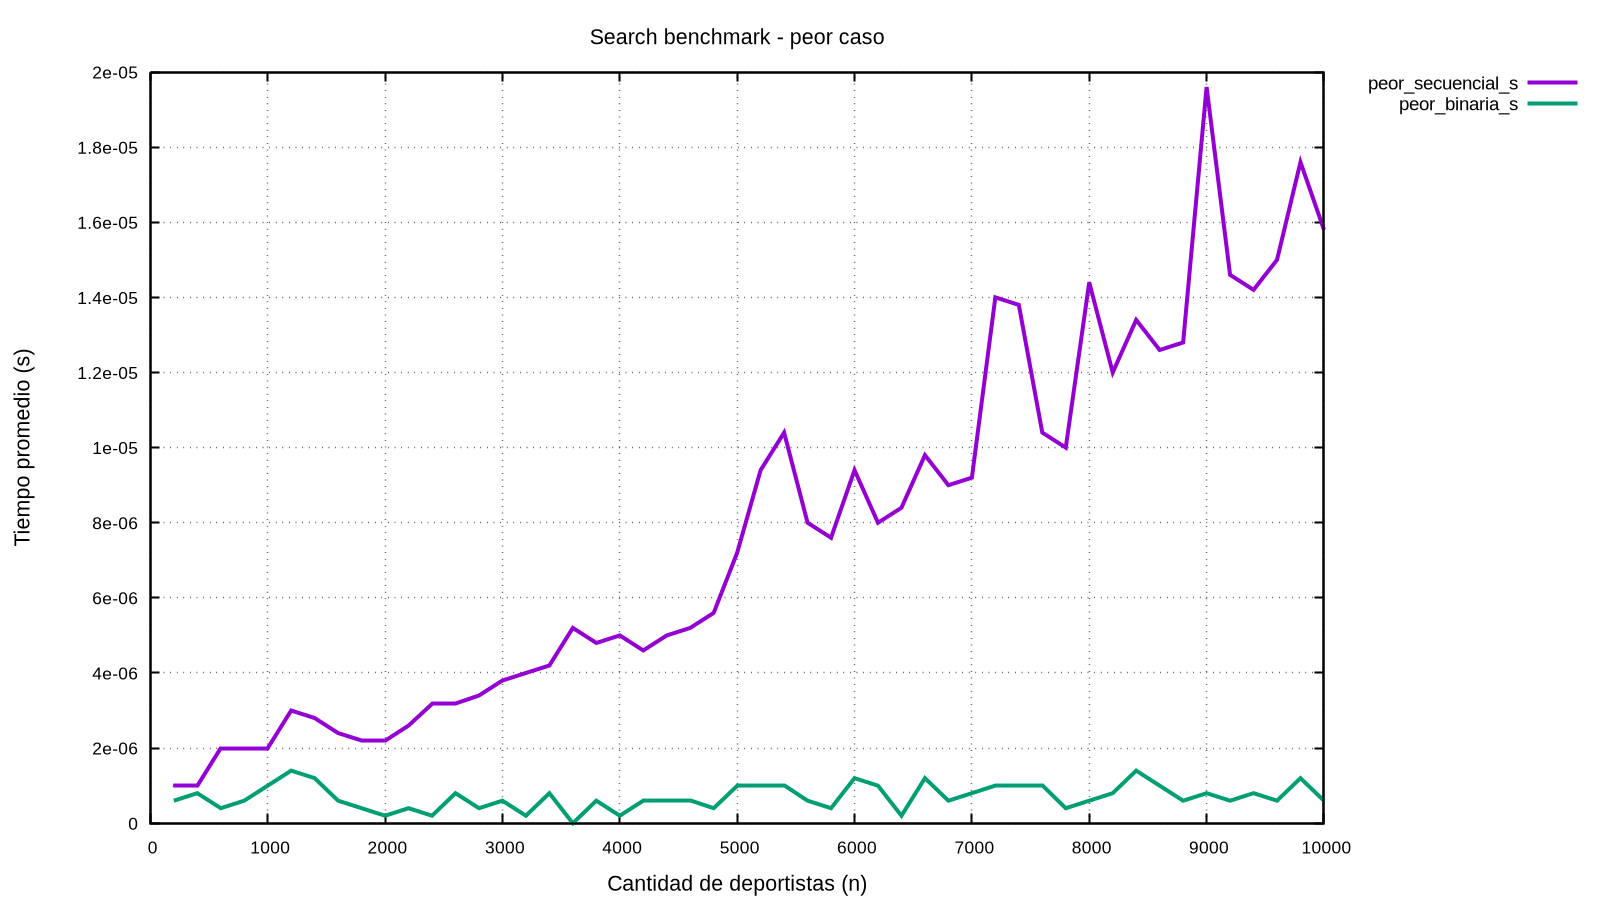
\includegraphics[width=0.95\textwidth]{Fig/search_worst_benchmark}
    \caption{Benchmark de búsqueda en peor caso}
    \label{fig:search_worst_benchmark}
\end{figure}

En la Figura \ref{fig:search_worst_benchmark} se aprecia que la búsqueda secuencial presenta una mayor demora que la búsqueda binaria iterativa en el peor caso. Tomando como referencia los extremos del experimento, la búsqueda secuencial pasa de \(8.0 \times 10^{-7}\) s en \(n=400\) a \(5.48 \times 10^{-5}\) s en \(n=20{,}000\), mientras que la búsqueda binaria iterativa se mantiene entre \(4.0 \times 10^{-7}\) s y \(8.0 \times 10^{-7}\) s. Esto significa que, al final del rango medido, la búsqueda secuencial tarda aproximadamente \(68\) veces más que la búsqueda binaria iterativa. Aunque existen pequeñas oscilaciones entre puntos consecutivos, la tendencia general coincide con la teoría: la búsqueda secuencial tiene costo \(O(n)\) al revisar todos los elementos cuando el ID buscado no existe, mientras que la búsqueda binaria iterativa mantiene un costo \(O(\log n)\) al dividir el espacio de búsqueda en cada iteración.

\subsection{Benchmark de ordenamiento: Mejor caso}
\begin{figure}[H]
    \centering
    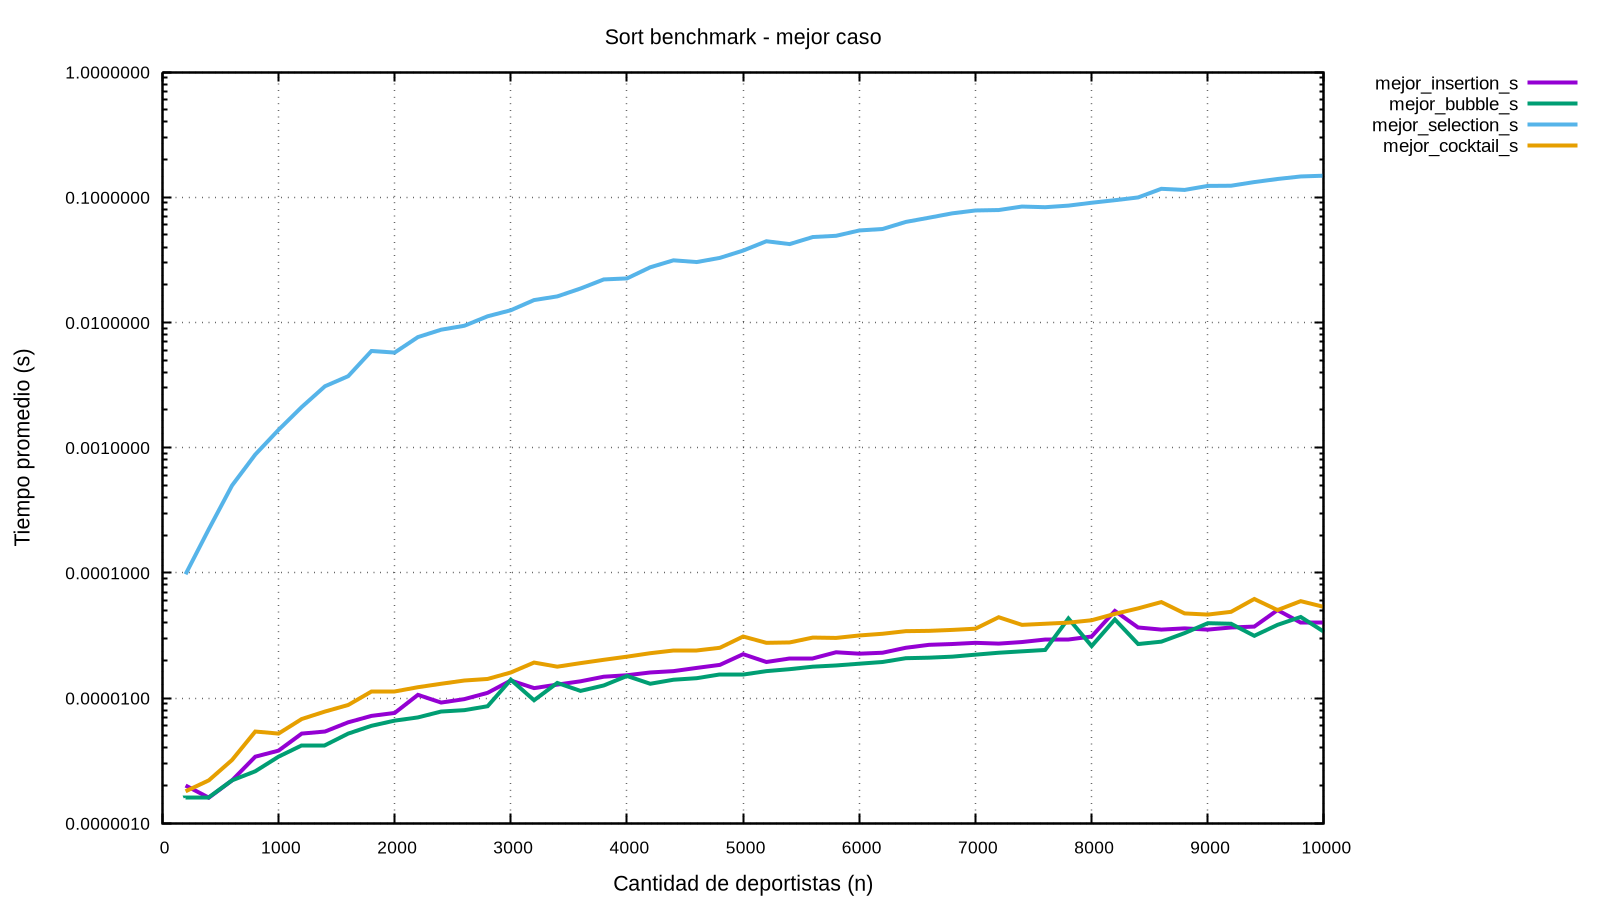
\includegraphics[width=0.95\textwidth]{Fig/sort_best_benchmark}
    \caption{Benchmark de ordenamiento en mejor caso}
    \label{fig:sort_best_benchmark}
\end{figure}

En la Figura \ref{fig:sort_best_benchmark}, Bubble Sort optimizado e Insertion Sort presentan los menores tiempos de ejecución, seguidos por Cocktail Shaker Sort, mientras que Selection Sort optimizado queda claramente por encima del resto. La diferencia es lo suficientemente grande como para justificar el uso de escala logarítmica en el eje vertical. En \(n=20{,}000\), Bubble Sort optimizado registra aproximadamente \(8.04 \times 10^{-5}\) s, Insertion Sort \(9.68 \times 10^{-5}\) s y Cocktail Shaker Sort \(1.10 \times 10^{-4}\) s, mientras que Selection Sort optimizado alcanza \(6.67 \times 10^{-1}\) s. Es decir, en este escenario Selection Sort optimizado resulta más de \(6{,}000\) veces más lento que los otros algoritmos de mejor desempeño. Este comportamiento es coherente con la teoría: Insertion Sort, Bubble Sort optimizado y Cocktail Shaker Sort se benefician de una entrada ya ordenada y se mantienen cercanos a \(O(n)\), mientras que Selection Sort optimizado conserva costo \(O(n^2)\) debido a que continúa realizando comparaciones sobre todo el arreglo.

\subsection{Benchmark de ordenamiento: Caso promedio}
\begin{figure}[H]
    \centering
    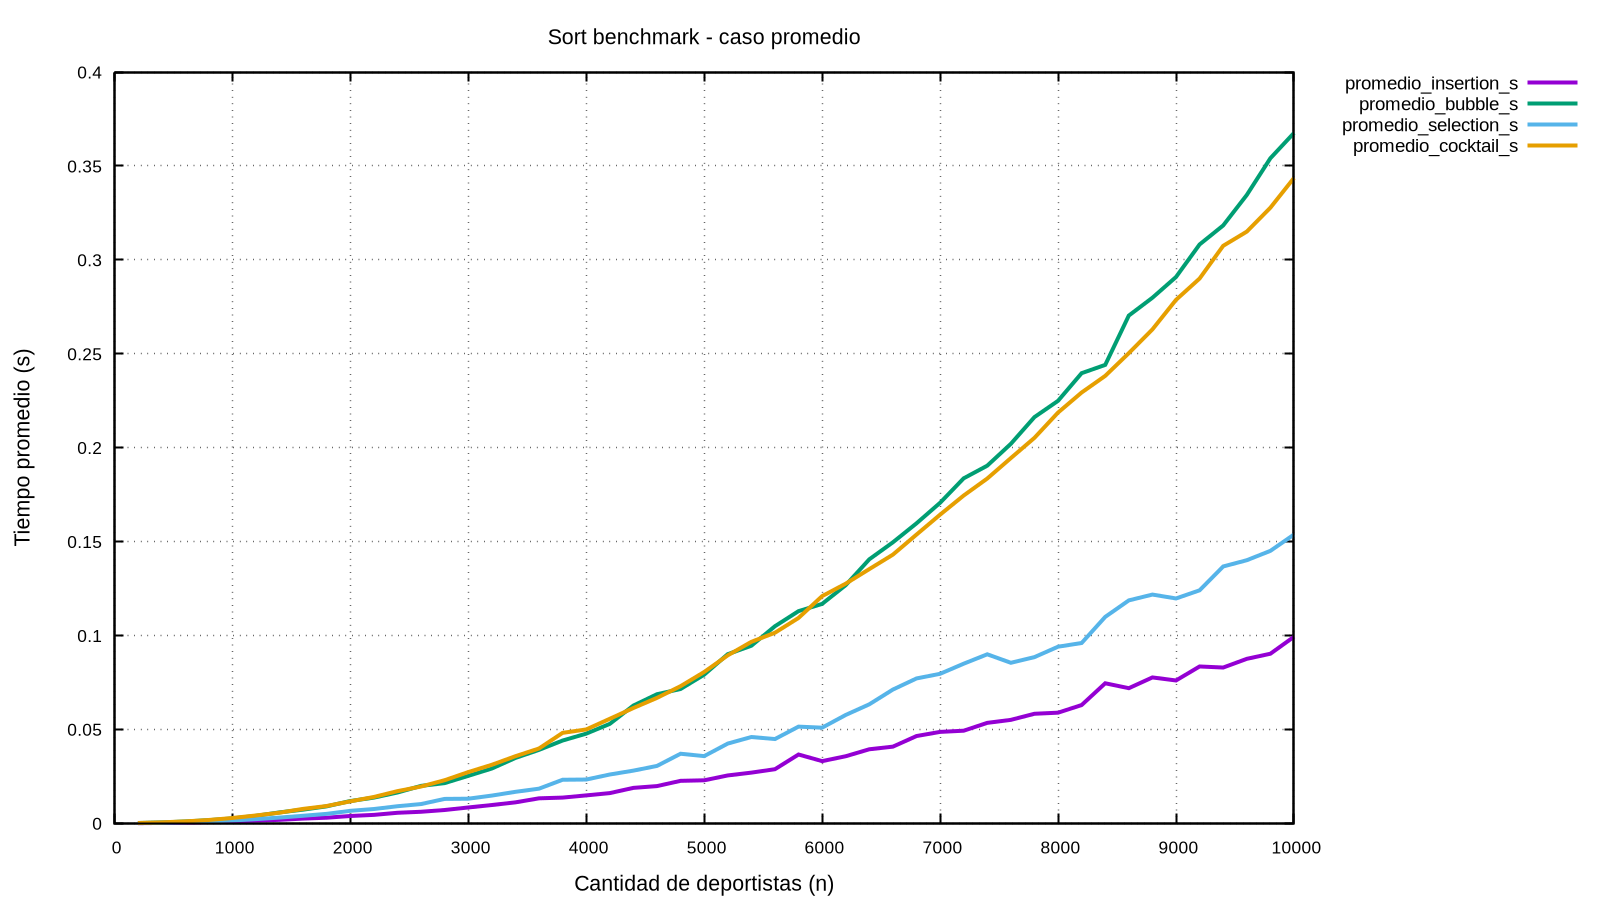
\includegraphics[width=0.95\textwidth]{Fig/sort_average_benchmark}
    \caption{Benchmark de ordenamiento en caso promedio}
    \label{fig:sort_average_benchmark}
\end{figure}

La Figura \ref{fig:sort_average_benchmark} muestra que Insertion Sort obtiene el mejor rendimiento en el caso promedio, seguido por Selection Sort optimizado, mientras que Bubble Sort optimizado y Cocktail Shaker Sort presentan tiempos mayores. En \(n=20{,}000\), Insertion Sort alcanza \(4.16 \times 10^{-1}\) s, Selection Sort optimizado \(6.64 \times 10^{-1}\) s, Cocktail Shaker Sort \(1.48\) s y Bubble Sort optimizado \(1.78\) s. En consecuencia, Insertion Sort es aproximadamente \(1.6\) veces más rápido que Selection Sort optimizado y más de \(4\) veces más rápido que Bubble Sort optimizado. En este escenario, los cuatro algoritmos mantienen complejidad \(O(n^2)\), pero se diferencian en la cantidad de comparaciones, desplazamientos e intercambios realizados. Insertion Sort logra un mejor comportamiento práctico al insertar cada elemento en su posición de forma relativamente eficiente, mientras que Selection Sort optimizado se mantiene competitivo por su menor cantidad de intercambios. Por su parte, Bubble Sort optimizado y Cocktail Shaker Sort aumentan más rápidamente su tiempo de ejecución debido a la mayor cantidad de movimientos necesarios sobre datos desordenados.

\subsection{Benchmark de ordenamiento: Peor caso}
\begin{figure}[H]
    \centering
    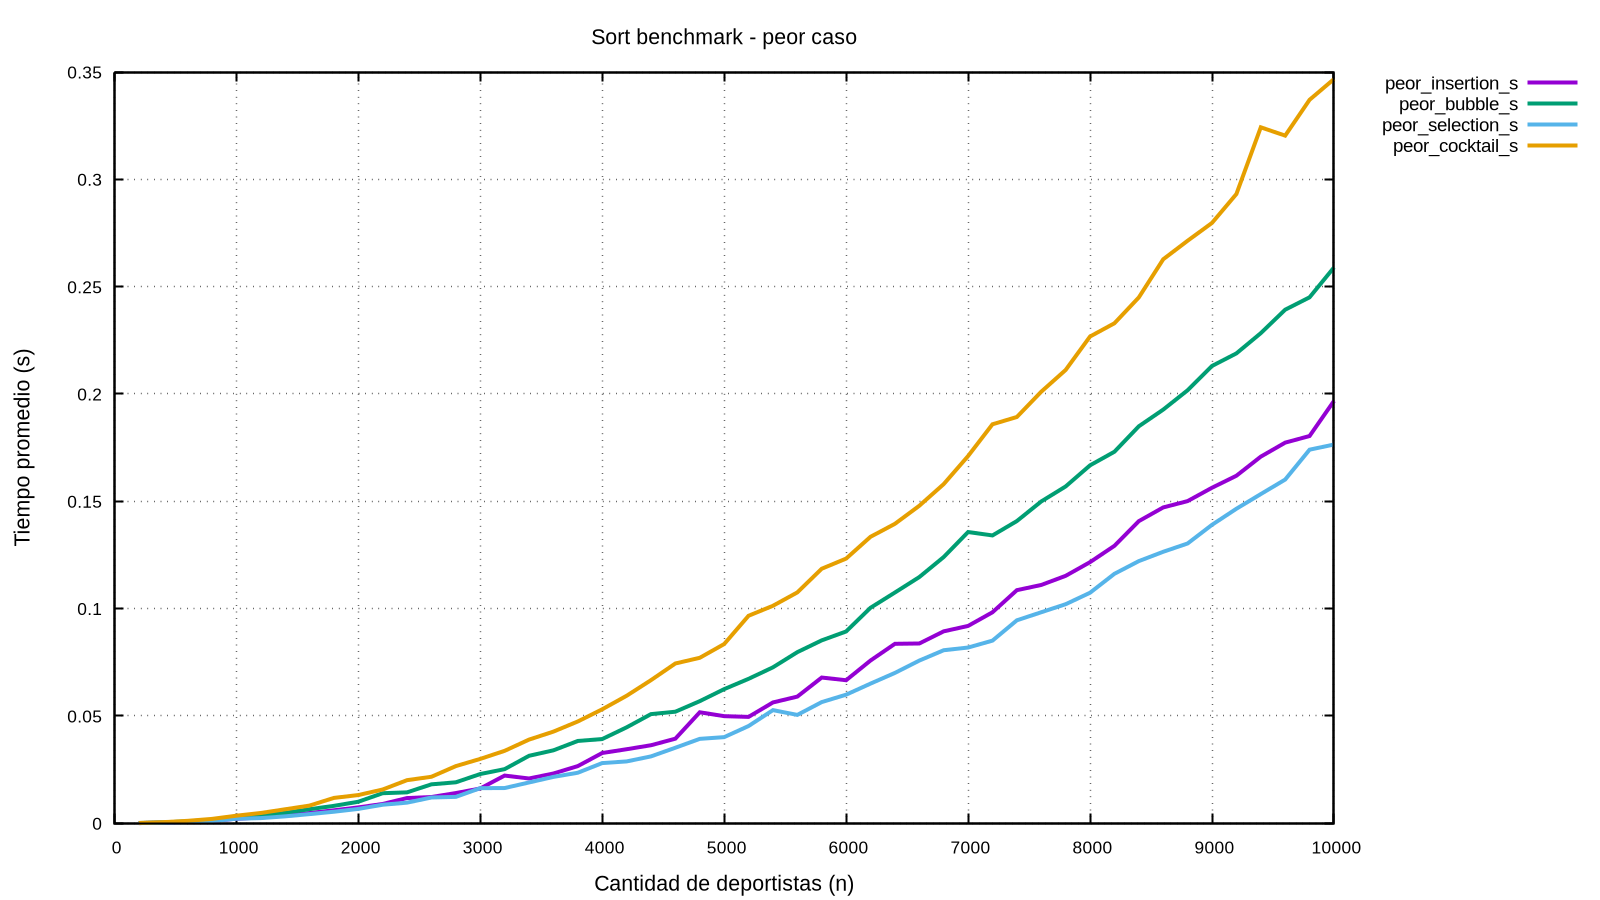
\includegraphics[width=0.95\textwidth]{Fig/sort_worst_benchmark}
    \caption{Benchmark de ordenamiento en peor caso}
    \label{fig:sort_worst_benchmark}
\end{figure}

En la Figura \ref{fig:sort_worst_benchmark} se observa que Selection Sort optimizado presenta los menores tiempos dentro del peor caso, seguido por Insertion Sort, mientras que Bubble Sort optimizado y Cocktail Shaker Sort son los más lentos, siendo este último el de mayor demora. En \(n=20{,}000\), Selection Sort optimizado registra \(7.76 \times 10^{-1}\) s, Insertion Sort \(8.84 \times 10^{-1}\) s, Bubble Sort optimizado \(1.14\) s y Cocktail Shaker Sort \(1.45\) s. Esto implica que, en el extremo del rango medido, Selection Sort optimizado es aproximadamente un \(12\%\) más rápido que Insertion Sort, un \(32\%\) más rápido que Bubble Sort optimizado y un \(47\%\) más rápido que Cocktail Shaker Sort. Teóricamente, los cuatro algoritmos conservan complejidad \(O(n^2)\) en este escenario, pero sus constantes de ejecución son distintas. Selection Sort optimizado mantiene un comportamiento más estable porque reduce el número de pasadas externas y realiza pocos intercambios, incluso cuando la entrada está invertida. Insertion Sort empeora por el aumento de desplazamientos necesarios, mientras que Bubble Sort optimizado y Cocktail Shaker Sort exhiben un crecimiento mayor debido a la gran cantidad de comparaciones e intercambios requeridos para reordenar completamente el arreglo.

\newpage
\subsection{Análisis general}
En términos generales, los resultados experimentales obtenidos son coherentes con el comportamiento teórico esperado para los algoritmos implementados. En el caso de búsqueda, la búsqueda binaria iterativa mostró un mejor rendimiento que la búsqueda secuencial en el peor caso, lo que coincide con sus complejidades \(O(\log n)\) y \(O(n)\), respectivamente. Esto confirma que, cuando los datos se encuentran ordenados, la búsqueda binaria iterativa resulta considerablemente más eficiente para tamaños de entrada crecientes.

En los algoritmos de ordenamiento también se observaron tendencias acordes a la teoría. En el mejor caso, Bubble Sort optimizado e Insertion Sort presentaron los menores tiempos, mientras que Selection Sort optimizado se mantuvo varios órdenes de magnitud por encima del resto debido a que continúa realizando una gran cantidad de comparaciones incluso cuando la entrada ya está ordenada. En el caso promedio, Insertion Sort obtuvo el mejor desempeño general, seguido por Selection Sort optimizado, mientras que Bubble Sort optimizado y Cocktail Shaker Sort presentaron mayores tiempos de ejecución. Finalmente, en el peor caso, Selection Sort optimizado mostró el comportamiento más estable, mientras que Bubble Sort optimizado y Cocktail Shaker Sort concentraron las mayores demoras.

En conjunto, estos resultados permiten concluir que no todos los algoritmos con la misma complejidad asintótica presentan el mismo rendimiento en la práctica. Aunque varios de ellos comparten complejidad \(O(n^2)\), las diferencias en la cantidad de comparaciones, desplazamientos, intercambios y precondiciones afectan directamente su desempeño real. De esta manera, el análisis experimental complementa la teoría y permite entender con mayor claridad las ventajas y limitaciones de cada algoritmo en distintos escenarios.

\subsection{Limitaciones del análisis experimental}
\begin{itemize}
    \item Los tiempos fueron medidos con \texttt{clock()}, por lo que en operaciones del orden de microsegundos aparecen pequeñas fluctuaciones entre puntos consecutivos.
    \item Los resultados dependen del hardware, del compilador, de la carga del sistema y del tamaño del conjunto de datos utilizado al momento de ejecutar los benchmarks.
    \item La búsqueda binaria iterativa se reporta sin incluir el tiempo de ordenamiento previo, por lo que sus resultados deben interpretarse como costo de búsqueda sobre datos ya ordenados y no como costo total de preparar y buscar.
    \item Los datos utilizados son sintéticos y el criterio de búsqueda evaluado fue únicamente el ID, por lo que las conclusiones describen este contexto experimental específico.
    \end{itemize}
